\chapter{Leçon 18: Erweiderung zu Leçon 7 - Dëschgeschier an Accessoiren}

\section{Neie Vokabulär / Nouveau Vocabulaire / New Vocabulary}

Dës Leçon ergänzt d'Leçon 7 un, andeems se sech op Objeten op engem Dësch an op Accessoiren, déi eng Persoun dréit, fokusséiert. \textit{Cette leçon complète la Leçon 7 en se concentrant sur les objets sur une table et sur les accessoires qu'une personne porte.}

\subsection{Dëschgeschier / Vaisselle et Couverts / Tableware}
\begin{itemize}
    \item \textbf{den Teller} (l'assiette / the plate)
    \item \textbf{d'Schossel} (le bol / the bowl)
    \item \textbf{d'Glas} (le verre / the glass)
    \item \textbf{d'Taass} (la tasse / the cup)
    \item \textbf{d'Karaff} oder \textbf{de Krou} (la carafe, le pot / the carafe, the jug)
    \item \textbf{d'Messer} (le couteau / the knife)
    \item \textbf{d'Forschett} (la fourchette / the fork)
    \item \textbf{de Läffel} (la cuillère / the spoon)
    \item \textbf{den Dësch decken} (mettre la table / to set the table)
\end{itemize}

\subsection{Accessoiren (ausser Kleeder) / Accessoires / Accessories}
\begin{itemize}
    \item \textbf{de Brëll} (les lunettes / the glasses)
    \item \textbf{de Sonnebrëll} (les lunettes de soleil / the sunglasses)
    \item \textbf{d'Ketten} (le collier / the necklace)
    \item \textbf{de Medaillon} (le médaillon, le pendentif / the medallion, the pendant)
    \item \textbf{den Ouerrank} (Pl.: \textbf{d'Ouerréng}) (la boucle d'oreille / the earring)
    \item \textbf{de Bracelet} (le bracelet / the bracelet)
    \item \textbf{de Rank} (la bague / the ring)
    \item \textbf{d'Aarmbandauer} oder \textbf{d'Auer} (la montre / the watch)
\end{itemize}

\section{Biller beschreiwen / Décrire des Images / Describing Pictures}

\subsection{Bild 1: E gedeckten Dësch / Une table mise / A set table}

\begin{figure}[h!]
    \centering
    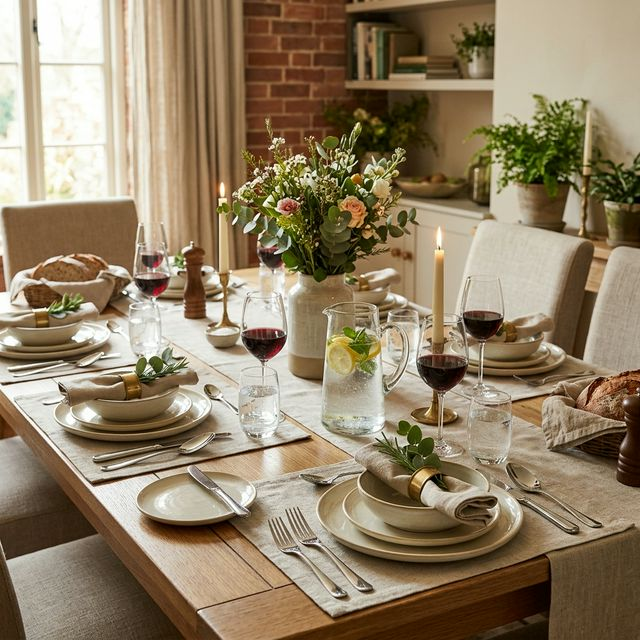
\includegraphics[width=0.8\textwidth]{vokab_300dpi/desch_geschier.png}
    \caption{E schéi gedeckten Dësch / Une table joliment dressée / A beautifully set table}
\end{figure}

\textbf{Beschreiwung (Lëtzebuergesch):}

Op dësem Bild gesi mir e schéi gedeckten Dësch fir e Mëttegiessen oder en Owesiessen. An der Mëtt steet eng grouss Karaff mat Waasser, Zitrounen a Peffermënzblieder. Ronderëm stinn elegant Wäiglieser an e puer Glieser mat Waasser. Fir jiddereen ass e wäissen Teller an eng kleng Schossel preparéiert, zesumme mam richtege Besteck: Messer, Forschett, a Läffel. D'Atmosphär ass ganz waarm a festlech, mat Käerzen an enger Vase mat Blummen an der Mëtt.

\textbf{Description (Français):}

Sur cette image, nous voyons une table joliment dressée pour un déjeuner ou un dîner. Au milieu se trouve une grande carafe avec de l'eau, des citrons et des feuilles de menthe. Autour se trouvent d'élégants verres à vin et quelques verres d'eau. Pour chacun, une assiette blanche et un petit bol sont préparés, ainsi que les couverts appropriés : couteau, fourchette et cuillère. L'atmosphère est très chaleureuse et festive, avec des bougies et un vase de fleurs au centre.

\textbf{Description (English):}

In this picture, we see a beautifully set table for a lunch or dinner. In the middle is a large jug with water, lemons, and mint leaves. Around it stand elegant wine glasses and some glasses of water. For everyone, a white plate and a small bowl are prepared, along with the right cutlery: knife, fork, and spoon. The atmosphere is very warm and festive, with candles and a vase of flowers in the center.

\vspace{1cm}

\subsection{Bild 2: Eng Fra mat Accessoiren / Une femme avec des accessoires / A woman with accessories}

\begin{figure}[h!]
    \centering
    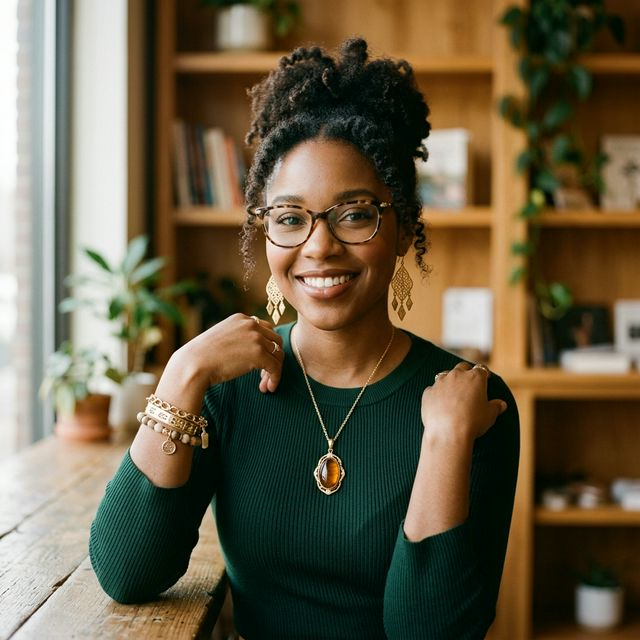
\includegraphics[width=0.6\textwidth]{vokab_300dpi/accessoire_fra.png}
    \caption{Portrait mat Accessoiren / Portrait avec des accessoires / Portrait with accessories}
\end{figure}

\textbf{Beschreiwung (Lëtzebuergesch):}

Dëst Bild weist e schéine Portrait vun enger jonker Fra, déi verschidden Accessoiren unhuet. Si huet en elegante Brëll un deen hir gutt steet. Ëm hiren Hals dréit si eng ganz markant gëlle Kette mat engem grousse Medaillon an der Mëtt. An den Ouere kënne mir detailléiert Ouerréng gesinn, déi liicht erofhänken. Um lénksen Aarm huet si en opfällege, gëllene Bracelet ronderëm d'Handgelenk. Si gesäit ganz houfereg aus a lächelt an d'Kamera.

\textbf{Description (Français):}

Cette image montre un magnifique portrait d'une jeune femme portant divers accessoires. Elle porte d'élégantes lunettes qui lui vont bien. Autour de son cou, elle porte un collier en or très marqué avec un grand pendentif au centre. À ses oreilles, nous pouvons voir des boucles d'oreilles détaillées qui pendent légèrement. Sur son bras gauche, elle porte un bracelet en or voyant autour du poignet. Elle a l'air très élégante et sourit à la caméra.

\textbf{Description (English):}

This image shows a beautiful portrait of a young woman wearing various accessories. She is wearing elegant glasses that suit her well. Around her neck, she wears a very striking gold necklace with a large pendant in the middle. In her ears, we can see detailed earrings that hang down slightly. On her left arm, she is wearing a conspicuous gold bracelet around her wrist. She looks very stylish and is smiling at the camera.

\vspace{1cm}

\subsection{Bild 3: Stillewen mat Schmuck / Nature morte avec des bijoux / Still life with jewelry}

\begin{figure}[h!]
    \centering
    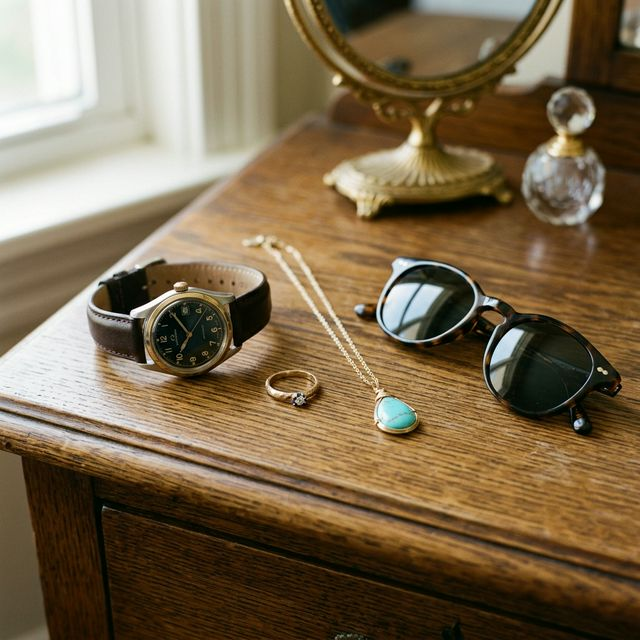
\includegraphics[width=0.8\textwidth]{vokab_300dpi/accessoire_aueren.png}
    \caption{Schmuck an Accessoiren / Bijoux et accessoires / Jewelry and accessories}
\end{figure}

\textbf{Beschreiwung (Lëtzebuergesch):}

Hei gesi mir eng Foto, wou verschidden Accessoiren ordentlech op engem hëlzene Miwwel (vläicht enger Komoud) leien. Op der lénker Säit ass eng klassesch Aarmbandauer mat engem bronge Liederband. An der Mëtt leien en delikate Medaillon un enger gëllener Ketten, an e schéine gëllene Rank. Riets dovu läit e moderne Sonnebrëll mat däischtere Glieser. Et ass eng typesch Zeen, ier ee sech de Moie fäerdeg mécht.

\textbf{Description (Français):}

Ici, nous voyons une photo où divers accessoires sont soigneusement disposés sur un meuble en bois (peut-être une commode). Sur le côté gauche se trouve une montre-bracelet classique avec un bracelet en cuir marron. Au centre se trouvent un délicat pendentif sur une chaîne en or et une belle bague en or. À droite de cela, il y a des lunettes de soleil modernes avec des verres foncés. C'est une scène typique avant de se préparer le matin.

\textbf{Description (English):}

Here we see a photo where various accessories are neatly laid out on a wooden piece of furniture (perhaps a dresser). On the left side is a classic wristwatch with a brown leather strap. In the center lie a delicate pendant on a gold chain and a beautiful gold ring. To the right of that are modern sunglasses with dark lenses. It is a typical scene before getting ready in the morning.
